% !TeX root = skripta-konstitutivni-vztahy.tex
% !TeX lastmodified = 2006-09-11

\subsection{Stavová rovnice ideálního plynu}
se obvykle zapisuje ve tvaru
\begin{equation}
	p v = r T,
\end{equation}
kde
\begin{description}
	\item[$p$] je tlak plynu,
	\item[$v$] je měrný objem plynu,
	\item[$r$] je měrná plynová konstanta,
	\item[$T$] je absolutní teplota.
\end{description}

Vynásobíme-li uvedenou rovnici molovou hmotností látky $M$, změní se na levé straně měrný objem plynu na molový objem plynu a~na pravé straně se změní měrná plynová konstanta na univerzální (molovou) plynovou konstantu $R_m$, jejíž hodnota je pro všechny ideální plyny stejná a~činí $R_m = \SI{8.3143 \pm 0.0012}{\joule\per\mole\per\kelvin}$.

Známý $p-V$ diagram izotermického (tj. hyperbola), resp. adiabatického (strmější adiabata) děje lze znázornit v~souřadnicích střední napětí $\sigma_s$ -- poměrná změna objemu $e$
\begin{figure}[H]
	\centering
	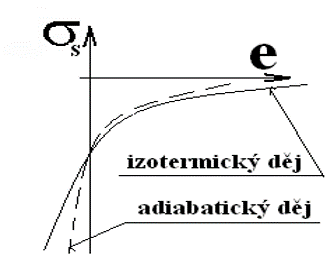
\includegraphics[height=4cm]{izotermicky-adiabaticky-dej}
	\caption{$\sigma_s-e$ diagram}
	\label{fig:izotermicky-adiabaticky-dej}
\end{figure}
